\section{Experiments}
\label{sec:experiments}
{First, we report \ours evaluation} on 3D online semantic mapping on two established datasets, one synthetic (Replica), and one real (ScanNetv2).
{Then, we present our \clipours evaluation} on semantic classification of images with ground-truth segmentation masks both on a dataset with multiple masks per image (ScanNet++) and with a single mask per image (ImageNet-S){, and against alternative methods integrated into \ours for 3D semantic mapping (Replica).}
%\ours was evaluated on 3D online semantic mapping on two standard datasets in the field, one synthetic (Replica), and one real (ScanNetv2).
%Our \clipours is evaluated on semantic classification of images with ground-truth segmentation masks both on a dataset with multiple masks per image (ScanNet++) and with a single mask per image (ImageNet-S).

{\boldparagraph{Implementation.} For \ours,} we implemented three different configurations {to show its flexibility}: (1)~\textbf{\ours-mapping}, that uses ground-truth camera poses, (2)~\textbf{\ours-Gaussian-SLAM}, {where we} integrate our contributions within Gaussian-SLAM~\cite{yugay2023gaussian}{, a SLAM method targeting novel-view synthesis and dense point cloud reconstruction, although not real-time}, and (3)~\textbf{\ours-ORB-SLAM2} for which we {integrate} {with ORB-SLAM2~\cite{mur2017orb}, a real-time feature-based SLAM system with loop-closure. While \ours-Gaussian-SLAM uses the center of 3D Gaussians as the dense point cloud \(\mathcal{P}\), for \textbf{\ours-ORB-SLAM2} we build a dense point cloud by registering the local point clouds from the RGB-D images}.
All three configurations use SAM2.1-l for 2D segmentation and SigLip ViT-SO400 for CLIP descriptors. %We also implement an \ours-mapping Lite with SAM1-H and CLIP ViT-H/14. 
%For more implementation details on \clipours and \ours  refer to~\cref{sup:imp}.
%
{\textbf{Our \clipours}} has 5 self-attention layers with 8 heads, {a 1152 latent dimension, with drop-out of 0.1, }and 4 layers MLP {with \(3\times 1152\) input/output neurons and \(\times4\) inverse bottleneck with Leaky ReLU activations.} {It was trained with 4 Nvidia V100 GPUs, using Pytorch, with AdamW optimizer, learning rate \(1\times10^{-6}\), gradient clipping at 1, and batch size of 512 per GPU,} for 15 epochs using the top 100 semantic labels from ScanNet++ 250 training set. {To compensate for class imbalance, in the loss we weight each element of the batch by the inverse of their class frequency in the training set.}

\boldparagraph{Baselines.}
We evaluate~\clipours against baselines that compute local CLIP descriptors~\cite{conceptfusion, gu2024conceptgraphs,hovsg} (using all of them SigLIP-SO400M) and Alpha-CLIP~\cite{sun2024alpha}, a state-of-the-art model developed to condition CLIP using masks.
{Additionally, we include two variations of our \clipours trained in the same setup, in order to validate its design: directly predicting the fused descriptor, and predicting only one weight per descriptor.} 
As detailed in \cref{sec:related}, existing semantic SLAM pipelines do not construct a 3D representation that can be evaluated using 3D metrics for open-set classes. 
%Instead, they either rely on 2D semantic representations~\cite{ji2024neds,zhai2024nis} or assume known 2D semantic labels within a closed vocabulary~\cite{zhai2024nis,li2024sgs}.
Thus, we compare \ours against similar 3D open-vocabulary online mapping systems, Concept-Graphs~\cite{gu2024conceptgraphs}, and OpenFusion~\cite{yamazaki2024open}; and the state-of-the-art 3D open-vocabulary offline baselines OpenScene~\cite{Peng2023OpenScene}, OpenNeRF~\cite{engelmann2024opennerf}, Open3DIS~\cite{nguyen2024open3dis} and HOV-SG~\cite{hovsg}.
Finally, we evaluate computational cost against Concept-Graphs, OpenFusion, HOV-SG and OpenNeRF, but exclude Open3DIS and OpenScene, as they rely on pre-processed 3D geometry and features.

\boldparagraph{Datasets.} 
ScanNet++~\cite{yeshwanthliu2023scannetpp} has 250 training and 50 validation indoor RGB+D scenes sequences. We use 2D rasterized masks for a total of 1.6M and 400k 2D instance samples respectively. Semantic classes are mapped into either the set of 100 most commons (used for training) or the full set of over 1.6k classes (used for evaluation).
ImageNet-S~\cite{gao2022luss} has a validation set of $\sim\!12$k images with 919 semantic labels. %Both datasets include ground-truth 2D/3D segmentation masks. 
%We assess \ours for open-vocabulary 3D semantic segmentation on ScanNetv2and Replica.
ScanNetv2~\cite{dai2017scannet} has a full validation set of 312 RGB+D sequences of real scenes (FVS). We also evaluate on the 5-scene subset used by HOV-SG (HVS). We use the original annotation set with 20 classes (ScanNet20) and the expanded set with 200 classes (ScanNet200~\cite{rozenberszki2022language}).
On Replica~\cite{replica19arxiv}, we use the standard 8-scene subset (\textit{office-0...4}, \textit{room-0...2}) and its 51 annotated classes.
%For more details on the datasets, refer to ~\cref{sup:datasets}.
\begin{table*}[ht]
\caption{3D semantic segmentation evaluation on Replica 51 classes, splitting by frequency tertiles: Head, Common and Tail.}
\label{tab:replica}
\centering
\setlength{\tabcolsep}{6.5pt}
\footnotesize
\begin{tabular}{l|ccc|cccccccc}
   \toprule
   & & \multirow[b]{2}{*}{\makecell{Geo-\\metry}}& \multirow[b]{2}{*}{\makecell{Camera pose / \\{ATE RMSE} {[cm]}}} & \multicolumn{2}{c}{All} & \multicolumn{2}{c}{Head} & \multicolumn{2}{c}{Common} & \multicolumn{2}{c}{Tail} \\
  \cmidrule(lr){5-6} \cmidrule(lr){7-8} \cmidrule(lr){9-10} \cmidrule(lr){11-12}
  Method & Online & &  & mIoU & mAcc & mIoU & mAcc & mIoU & mAcc & mIoU & mAcc \\
  \midrule
  OpenScene~\cite{Peng2023OpenScene} (Distilled)&\xmark& GT & GT & 14.8 & 23.0 & 30.2 & 41.1 & 12.8 & 21.3 & 1.4 & 6.7 \\
  OpenScene~\cite{Peng2023OpenScene} (Ensemble) &\xmark& GT & GT & 15.9 & 24.6 & 31.7 & 44.8 & 14.5 & 22.6 & 1.5 & 6.3 \\
  OpenNeRF~\cite{engelmann2024opennerf}         &\xmark  & Est.& GT & 20.4 & 31.7 & 35.4 & 46.2 & 20.1 & 31.3 & 5.8 & 17.6 \\
  HOV-SG~\cite{hovsg}                            &\xmark & Est. &GT &  22.5 & 34.2 & 35.9 & 44.2 & \rd 23.6 & \nd 42.3 & 8.0 & 16.1  \\
  Open3DIS~\cite{nguyen2024open3dis} (SigLip) &\xmark & GT & GT & 25.6 & \nd 38.7 & \fs 49.7 & \fs 64.4 & 22.1 & \fs 42.4 & 4.9 & 9.4 \\ \hdashline \noalign{\vskip 1pt}
  %O$_2$V-mapping~\cite{tie20242}             &\cmark & GT & Est. & 7.8 & 13.9 & 19.3 & 27.5 & 4.0 & 6.7 & 0.1  & 7.5 \\
  Concept-Graphs~\cite{gu2024conceptgraphs}             &\cmark  & Est. & GT & 16.7 & 33.7 & 27.3 & 39.1 & 15.1 & 35.4 & 4.4  & \fs 26.8 \\
  %Concept-Graphs-Detect~\cite{gu2024conceptgraphs}             &\cmark & GT & Est. & 13.4 & 36.9 & 21.3 & 42.2 & 13.9 & \fs 39.9 & 4.5  & \fs 29.3 \\
  Open-Fusion~\cite{yamazaki2024open}             &\cmark & Est. & GT & 20.5 & 34.8 & 37.9 & 51.7 & 14.0 & 30.3 & 9.8  & \rd 22.2 \\[0.8pt]  
  %\ours-mapping Lite (ours)                &\cmark & GT & Est. & 22.8 & 35.5 & 35.2 & 45.0 & 22.1 & \fs 44.6& \rd 11.0 & 16.9 \\[0.8pt]
  \textbf{\ours-mapping (ours)}                          &\cmark & Est. & GT & \nd 27.0 & \fs 39.1 & \nd 45.0 & \nd 59.9 & \fs 25.1 & 38.5 & \rd 11.0 & 18.8   \\ %[0.8pt]
  \hdashline \noalign{\vskip 1pt}
  \textbf{\ours-Gaussian-SLAM (ours)}                                         & \cmark & Est. &  \fs 0.6& \fs 27.1 & \rd 38.6 & \rd 44.1 & 58.0 & \nd 25.0 &\rd 39.0 & \fs 12.1 & 18.9   \\ 
  \textbf{\ours-ORB-SLAM2  (ours)}                                     &\cmark & Est. & \nd1.9 & \rd 25.6 &  39.0 & 43.0 & \rd 59.1 & 21.6 & 38.3 & \fs 12.1 & \rd 19.6   \\ 
  %\ours-ORB-SLAM2  (ours) w/o lc                                    &\cmark &Est.& Est. & 25.5 &  38.8 & 43.2 & 58.9 & 22.2 & 39.1 & 11.0 & 18.5   \\ 
  \bottomrule
\end{tabular}
\end{table*}
\begin{table*}[ht]
\centering
  \caption{3D semantic segmentation on ScanNetv2 with frequency weighted metrics on 5 (HVS) and all 312 val. scenes (FVS).}% \ours outperforms both offline and online baselines, in particular for frequency-weighted metrics and for the ScanNet200 set, both  }%
  \label{tab:scannetv2}
\footnotesize
\setlength{\tabcolsep}{4.0pt}  %{3.5pt} % column spacing5
\begin{tabular}{cl|ccc|ccccccccc}
  \toprule
    &&&\multirow[b]{2}{*}[5pt]{\makecell{Geo-\\metry}}& \multirow[m]{2}{*}{\makecell{Camera pose / \\ATE RMSE [cm]}} & \multicolumn{4}{c}{ScanNet20} & &\multicolumn{4}{c}{ScanNet200} \\ \cline{6-9}  \cline{11-14}
  &Method &Online & & & mIoU & mAcc & f-mIoU & f-mAcc & & mIoU & mAcc & f-mIoU & f-mAcc  \\
  \midrule
  \multirow{10}{*}{
\rotatebox[origin=c]{90}{HVS}} & Open3DIS~\cite{nguyen2024open3dis} (SigLip)   &\xmark &GT&GT& \rd 37.3 & \nd 52.8 & \rd 57.0 & \rd 67.9 && \fs 17.8 & \nd 23.7 &  27.9 & 34.1\\
  
  &OpenScene(Ensemble)~\cite{Peng2023OpenScene}   &\xmark &GT&GT & \fs 44.6 & \fs 61.9 & \fs 57.6 & \fs 71.0 & & 9.4 & 12.6 & 27.8 & 32.0\\
  &HOV-SG~\cite{hovsg}  &\xmark & Est.&GT & 34.4 & \rd 51.1 & 47.3 & 61.8 && 11.2 & 18.7 & 27.7 & 37.6 \\[0.8pt]
  \cdashline{2-14} \noalign{\vskip 1pt}
  %&Concept-Graphs-Detect~\cite{gu2024conceptgraphs}   &\cmark &GT& Est. & 22.4 & 41.7 & 30.5 & 43.2 & & 7.0 & 15.6 & 20.5 & 29.2 \\
  &Concept-Graphs~\cite{gu2024conceptgraphs}   &\cmark & Est. &GT& 17.1 & 29.1 & 26.0 & 33.1 & & 6.0 & 11.7 & 21.4 & 27.7 \\
  &Open-Fusion~\cite{yamazaki2024open}    &\cmark &Est. &GT& 30.1 & 39.9  & 54.1  & 68.1  & & 8.6 & 12.8 & \nd 38.4 & \rd 47.9  \\[0.8pt]
  \cdashline{2-14} \noalign{\vskip 1pt}
  %
  %&\ours-mapping-Lite (ours) &\cmark &GT&Est.& 25.6 & 43.8 & 32.4 & 43.8 && \rd 14.7 & \rd 22.9 &  27.9 & 37.2\\
  &\textbf{\ours-mapping (ours)} &\cmark &Est.& GT&\nd 38.1 & 50.5 & \fs 57.6 & \nd 70.5 && \nd 17.2 & \fs 25.3 & \fs 45.4 & \fs 56.4\\
  &\textbf{\ours-Gaussian-SLAM (ours)}             &\cmark&Est.&\nd{23.7}& 29.3 & 41.1 & 43.0 & 59.5&&  11.8 & 18.8 & 30.1 & 42.6 \\
  &\textbf{\ours-ORB-SLAM2 (ours)} &\cmark &Est.& \fs{21.5}& 31.3 & 45.2 & 45.8 & 61.2 && \rd 13.6 & \rd 22.2 & \rd 38.2 & \nd 51.0 \\
  &{\bf \ours-ORB-SLAM2 w/o loop clos.} &\cmark &{Est.}& \rd{30.2}& {23.6} & {34.5} & {41.4} & {56.9} && {10.3} & {17.3} & {33.2} & {46.0} \\
  \midrule
  \multirow{3}{*}{
\rotatebox[origin=c]{90}{FVS}}  & Open3DIS~\cite{nguyen2024open3dis} (SigLip)  &\xmark &GT&GT& \rd 24.7 & \rd 40.9 & \rd 32.5 & \rd 45.3 & & \rd 9.4 & \rd 17.0 & \rd 22.9 & \rd 32.2 \\[0.8pt]
  &OpenScene(Ensemble)~\cite{Peng2023OpenScene}  &\xmark &GT&GT& \fs 47.0 & \fs 70.3 & \fs 57.7 &\fs 69.8 & & \nd 11.6 & \nd 22.8 & \nd 24.5 & \nd 29.2 \\
  \cdashline{2-14} \noalign{\vskip 1pt}
  %
  & \textbf{\ours-mapping (ours)} &\cmark&Est.&GT& \nd 37.3 & \nd 58.9 & \nd 55.13 & \nd 69.4& & \fs 17.4 & \fs 35.9 & \fs 44.3 & \fs 57.8\\
  \bottomrule
  \end{tabular}
  \vspace{-5pt}
\end{table*}

\boldparagraph{Metrics.} 
Semantic classification is evaluated using \emph{mean Intersection Over Union} (mIoU) and \emph{mean Accuracy} (mAcc) on ScanNet++, while on ImageNet-S we report the standard Top-1 and Top-5 mAcc. While we assess \clipours in 2D to isolate other factors, the full \ours is evaluated in 3D by labeling the vertices of ground-truth meshes and comparing them against ground-truth 3D labels.
For Replica, following OpenNeRF~\cite{engelmann2024opennerf}, we report mIoU and mAcc, categorizing labels into tertiles based on their frequency (\emph{head}, \emph{common}, and \emph{tail}). 
In ScanNetv2, we further present metrics weighted by the label frequency in the ground truth (f-mIoU and f-mAcc).
Additionally, we analyze our computational footprint.
We measure wall-clock time required to optimize Replica scenes, as well as mean and max GPU vRAM and max system RAM usage (in GB).
 %For \ours, we also report the final representation size (in MB) and the time to process each keyframe (KFPS).
Each table highlights \colorbox{Green!25}{\textbf{first}}, \colorbox{SpringGreen!45}{second}, and \colorbox{Yellow!30}{third} best results.

%------------------------------------------------------------------------------
\subsection{3D Semantic Segmentation}
\label{sec:sem_seg_exp}
%------------------------------------------------------------------------------
%

\boldparagraph{Replica.} \cref{tab:replica} presents segmentation results for all our \ours configurations alongside relevant baselines. \ours outperforms all baselines in the aggregated mIoU and mAcc (`All' column).
\ours-Gaussian-SLAM and \ours-ORB-SLAM2 surpass both offline and online mapping algorithms.
This is particularly noteworthy since both implementations estimate camera poses and scene geometry, whereas all baselines (indicated in the table) rely either on ground-truth geometry, camera pose, or both.  
%Despite using different camera trackers, both implementations produce sharp and accurate reconstructions, demonstrating that tracking variations do not significantly impact our pipeline.
Thanks to the strong generalization of our \clipours, all \ours implementations have a significantly better mIoU on \emph{tail} categories, which demonstrates less false-positives.
%
%As a result, \ours-mapping Lite slightly outperforms the more computationally expensive HOV-SG using the same backbones, and is $+15$ points better than O$_2$V, the only other approach that estimates online the 3D semantic representation. 
%\newline
As shown in \cref{fig:replica}, \ours effectively segments and classifies 3D instances, such as chairs and tables, that other baselines often misclassify due to the excessive context information incorporated into CLIP descriptors.
\ours even outperforms the ground truth in some instances.
For example, in "office4" (top left of \cref{fig:replica}), the ground-truth label for the table is missing, and one chair is misclassified as the floor.
This underscores the advantage of open-set pipelines, particularly in situations where previous SLAM algorithms, which rely on known 2D semantics~\cite{li2024sgs, zhai2024nis}, would fail.

\boldparagraph{ScanNetv2.} Results, summarized in ~\cref{tab:scannetv2}, show how \ours-mapping matches HOV-SG, and even Open3DIS in the set ScanNet20.
On the harder set ScanNet200, \ours-mapping has a similar performance to Open3DIS in mIoU, although it is significantly better in terms of f-mIoU and f-mAcc.
OpenScene does achieve the best performance on ScanNet20. 
Nevertheless, its significant drop when using the extended set of classes highlights a weaker generalization capabilities than \ours and other baselines.
%Qualitative analysis, see bottom \cref{fig:scannetv2}, show how the three models (\ours-mapping, HOV-SG, and Open3DIS) struggle misclassifying and misegmenting several objects.
%\ours mapping labels part of the table as counter and over segments a window. 
%HOV-SG is predicting parts of the chairs as \textit{picture} and classifying most of the counter and furniture as \textit{wall}.
%Open3DIS completely misclassified the table as \textit{counter} and a cabinet as \textit{refrigerator}.

{\boldparagraph{SLAM comparison.}} The difference between \ours's two SLAM versions and \ours-mapping is bigger in ScanNetv2 than in Replica (compare \cref{tab:replica} and \cref{tab:scannetv2}), due to image blur and noisy depths in ScanNetv2.
%Gaussian-SLAM optimizes its 3D Gaussian Splatting representation generating a sparse {point cloud} resulting in a coarse 3D segmentation. 
{Gaussian-SLAM benefits from a more complex strategy for densification and pruning of the 3D point cloud, outperforming our simpler depth unprojection in Replica.
However, while its camera tracking works flawlessly there, it does struggle in ScanNetv2 noisier images, where loop-closure plays a key role.
}
Comparing \ours-ORB-SLAM2 w/o and w/ loop-closure, \cref{tab:scannetv2}, shows the importance of this feature. {Further, \cref{fig:loop_closure} illustrates the loop closure correction over} inconsistent reconstructions with repeated semantic instances, caused by odometric drift.

\begin{figure}
    \centering
    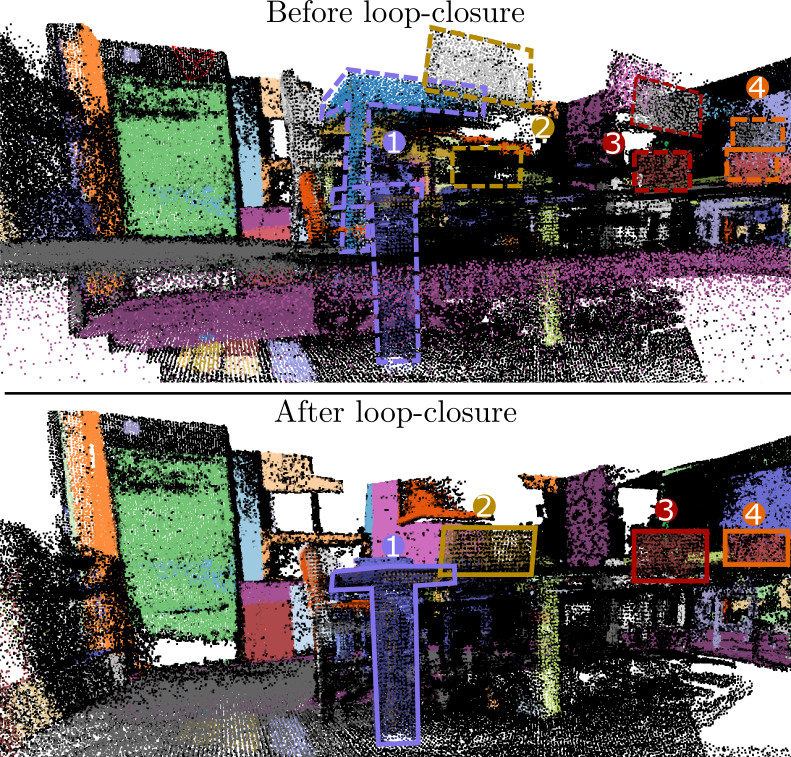
\includegraphics[width=\linewidth]{figures/images/loop_closure.png}
    \caption{{\textbf{Visualization of OVO-ORB-SLAM2 loop closure on  ``scene0011\_00'' (ScanNet)}. We highlight four instances split due to tracking drift and effectively merged after loop-closure by our semantic fusion.}}
    \label{fig:loop_closure}
\end{figure}
\begin{table}[tb]
  \caption{Runtime statistics on Replica with 2k frames per scene.}% \ours ranks second overall, offering an effective balance between accuracy and computational footprint.}
  \label{tab:time}
  \centering
  \footnotesize
  \setlength{\tabcolsep}{11.7pt}  %{8pt} % column spacing
  \begin{tabular}{lrrr}
    \toprule
           & vRAM & RAM & Time \\
    Method & Avg / Max & Max & Avg \\
    \midrule
    HOV-SG~\cite{hovsg}                  & \rd 6 / 12 GB &  139 GB &  $\sim$11h\\
    OpenNeRF~\cite{engelmann2024opennerf} & 4 / 22 GB & 44 GB & $\sim$20m\\ \hdashline    
    %O$_2$V~\cite{tie20242}                & 19 / 23 GB & \nd 17 GB & \rd $\sim$1h30m \\
    Open-Fusion~\cite{yamazaki2024open}                &  \fs 3 /\phantom{2} 4 GB & \fs 6 GB & \fs $\sim$3m \\
    %CG-Detect~\cite{gu2024conceptgraphs}                & \rd 6 / 10 GB & \nd 9 GB & \nd $\sim$6m \\
    CG~\cite{gu2024conceptgraphs}                &  \rd 7 / 11 GB & 16 GB &  $\sim$16m \\
    \ours-mapping (ours)                  & \nd 4 / \phantom{2}8 GB & \rd  12 GB & \nd $\sim$6m \\
    \bottomrule
  \end{tabular}
\end{table}

\boldparagraph{Computational footprint.}
Despite OpenFusion being \(2\times\) faster than \ours, thanks to using SEEM instead of SAM+SigLIP, ~\ours achieves a better balance between speed and performance. It is still \(2.5\times\) faster than Concept-Graphs, $3\times$ faster than OpenNerf and $80\times$ faster than HOV-SG, as shown in \cref{tab:time}. 
In contrast with HOV-SG, that relies on an expensive hierarchical merging of segments, requiring almost \(\times10\) more RAM, ~\ours shows a lower RAM and GPU vRAM usage that enables its use on consumer devices.
%Additional results, in \cref{tab:runtime}, show that \ours-mapping runs at $0.5$--$1$ keyframes per second on both Replica and ScanNetv2. 
{\ours-ORB-SLAM2 takes on average $0.67$ seconds per keyframe on Replica and ScanNetv2, spiking up to $1.4$ seconds for the slowest frame, and up to up to 2.5 and 6.1 seconds after loop closure on ``scene0011\_00'' and ``scene0231\_00'' respectively. This is compatible in our experiments with a conservative keyframe creation policy of 1 keyframe every 10 frames.% With our configuration segmenting 1 keyframe every 10 frames, OVO-ORB-SLAM2 runs at 14.8 FPS
}
Therefore, it is compatible with real-time SLAM pipelines, in which the critical camera tracking runs at video rate while the mapping runs at lower frequencies.
%

%Despite achieving state-of-the-art results on 3D semantic segmentation, \ours's instance detection and tracking has margin for improvement. 
%As demonstrated, \ours-mapping can be integrated into SLAM pipelines with real-time camera tracking. However, \ours operates at $0.5-1$ frames per second, introducing a slight delay in the semantics. Moreover, while \clipours generalizes better than the baselines, it still exhibits a slight bias toward the most frequent CLIPs and categories.
%A more robust training approach, involving a broader set of classes and incorporating semantic properties can enhance its capabilities.
%------------------------------------------------------------------------------
\subsection{{CLIP Merging}}
\label{sec:clipmerger_eval}
%------------------------------------------------------------------------------
In \cref{tab:clipmerging_imagenet}, we report evaluation on ImageNet-S, including also Alpha-CLIP, and on which both HOV-SG's and Concept-Fusion's merging approaches are equivalent to just computing the global descriptor due to there being only one mask per image.
\cref{tab:clipmerging} presents 2D semantic classification results on unseen scenes from ScanNet++, {using} the expanded label set {of 1.6k}, of our \clipours vs. HOV-SG's and Concept Fusion's (CF) CLIP merging, and the simpler mask crop used by Concept-Graphs. 

\begin{table}[ht!] 
    \caption{ImageNet-S semantic classification accuracy.}
    \label{tab:clipmerging_imagenet}
    \centering
\footnotesize
\setlength{\tabcolsep}{9.2pt}  % {5.2pt} % column spacing
\begin{tabular}{lcc}
    \toprule
    Method         &  Top-1 mAcc & Top-5 mAcc \\
    \midrule
    Alpha-Clip (ViT-L/14@336)\cite{sun2024alpha}     & 77.6               & 94.1               \\
    SigLIP-SO400M\cite{zhai2023siglip}     & \nd 82.5               & \nd 95.7               \\
    Mask crop      & \rd 80.3               & \rd 93.4               \\
    \textbf{Our CLIP merging}   & \fs 84.8               & \fs 96.6               \\
    \bottomrule
    \end{tabular}
 \end{table}
 %
 %
\begin{table}[ht]
\vspace{-5pt}
    \caption{2D Open vocabulary semantic classification on ScanNet++.}
    \label{tab:clipmerging}
\centering
\footnotesize
\setlength{\tabcolsep}{7.0pt} %{7pt} % column spacing
\begin{tabular}{lcccc}
\toprule
Method & mIoU & mAcc & f-mIoU &  f-mAcc\\\midrule
Concept-Fusion\cite{conceptfusion} & 8.6 & \fs 17.0 &  10.0 &  12.8 \\
Mask crop & 8.5 & \fs 17.0 &  10.0 &  12.8 \\
HOV-SG merging\cite{hovsg} & \nd 9.4 & \rd 15.9 & \rd 12.8 & \rd 15.9\\
\bf Our \clipours  & \fs 9.5 &   14.3 &\nd 36.9 & \nd 49.4 \\
\midrule
{\bf \textit{\clipours variations}} \\
{- fused } &  6.2 &  11.6 & \fs 40.0 & \fs 56.7 \\
{- per-descriptor} &  9.0 & \rd 15.6 &  12.7 & \rd 15.9 \\
\bottomrule
\end{tabular}
\end{table}
%
%
\begin{table}[h!]
%\vspace{-4pt}
\centering
    \footnotesize
    \setlength{\tabcolsep}{1.7pt} % column spacing
   \caption{{3D Open-Vocabulary Semantic metrics on Replica of OVO-mapping with alternative CLIP merging.}}\label{tab:replica_ablation}
\begin{tabular}{lccccccccc}
\toprule
 &  \multicolumn{2}{c}{All} && \multicolumn{2}{c}{Seen} && \multicolumn{2}{c}{Unseen} \\ \cline{2-3} \cline{5-6} \cline{8-9} 
 &  mIoU & mAcc & &mIoU & mAcc && mIoU & mAcc & \\ 
 \midrule
w/ HOV-SG's fusion & \nd 20.3 & \rd 38.1 && 22.3 & 45.1&& \fs 18.3& \fs 30.9  \\
\textbf{w/ our \clipours} & \fs 27.0 & \fs 39.1 && \fs 36.7 & \fs 54.7 && \nd 16.9 & \nd 22.8\\% \hline 
\midrule
\bf \textit{w/ \clipours variations} & & &\\
- fused & \rd20.2 & 33.2 && \nd32.2 & \nd52.5 && 0.8 & 1.2\\
- per-descriptor & \rd 20.2 & \nd38.2 && \rd26.6 &\rd48.6 && \rd 13.6 & \nd 27.4\\
\bottomrule
\end{tabular}
\end{table}
%
Overall, ours outperforms baselines, particularly in frequency-weighted metrics{, although with slightly worse mAcc in ScanNet++.}
Alpha-CLIP performs worse than simpler approaches like our~\clipours. Using a better backbone (SigLIP-SO400M vs ViT-L/14) outperforms a significantly more expensive fine-tuning (our trained two day on 4 V100 vs their on 128 A100 GPUs). 

{Regarding alternatives, the per-descriptor weights predictor achieves a similar performance to HOV-SG, while directly predicting a fused descriptor achieves better frequency-weighted metrics but significantly worse overall ones, which indicates overfitting.}
{This is further validated evaluating OVO-mapping in Replica, \cref{tab:replica_ablation} using HOV-SG's merging approach, and the alternatives to our \clipours. The fused predictor performance collapses in classes not seen during training, while our proposed \clipours has a slightly worse performance than HOV-SG's, while being significantly better on the known classes. 
The per-CLIP weights is unable to match the performance, highlighting the impact of per-dimension weights.}

Finally, we highlight in \cref{fig:gen_queries} how our \clipours preserves their rich semantic encoding, allowing our merged CLIPs to generalize to zero-shot complex language queries.
%These qualitative examples demonstrate how our merged CLIP vectors retain object properties and affordances beyond the training distribution.
For instance, our descriptors  distinguish between two trash bins based on a recycling symbol on one of them, despite both being labeled just as \textit{bin} in the ground truth.
%Unlike previous offline methods, \ours enables real-time querying of the 3D representations while they are being estimated online. 

\subsection{{Limitations}}\label{sec:limitations}
{Despite OVO state-of-the-art results on 3D indoor semantic segmentation, generalization to outdoor large-scale scenes may face challenges such as different class distributions, illumination and blur, and higher tracking errors.
Our semantic fusion at loop closure effectively corrects odometric drift. However, it sometimes misses instances that should be fused, something that may be fixed by a richer and more accurately localized set of features.
We also observed in \clipours a slight bias towards classes seen at training, which may be solved with larger training sets.}
